\documentclass{standalone}
\usepackage{tikz}
\usepackage{ctex,siunitx}
\usepackage{tkz-euclide}
\usepackage{amsmath}
\usetikzlibrary{patterns, calc}
\usetikzlibrary {decorations.pathmorphing, decorations.pathreplacing, decorations.shapes,}
\begin{document}
\small
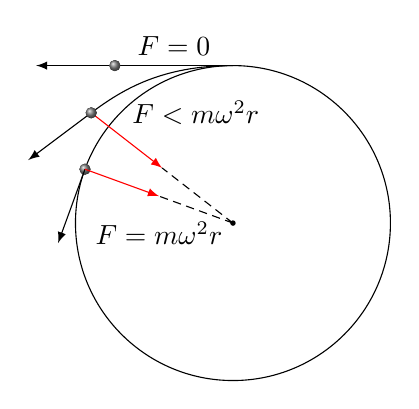
\begin{tikzpicture}[>=latex,scale=1]
  \draw(0,0)circle(2);
  \draw[->](0,2)--++(-1.5,0)node[midway,above]{$F=0$}--++(-1.0,0);
  \fill(0,0)circle(1pt);
  \fill[ball color=gray](-1.5,2)circle(2pt);
  \fill[ball color=gray](160:2)circle(2pt);
  \draw[->](160:2)--++(250:1.0);
  \draw[thin,densely dashed](0,0)--(160:1)(0,0)--(-0.9,0.7);
  \draw[->,red](160:2)--++(-20:1.0)node[below=2mm,text=black]{$F=m\omega^2r$};
  \draw[->,red](-1.8,1.4)node[right=4mm,text=black]{$F<m\omega^2r$}--(-0.9,0.7);
  \draw[->](90:2)..controls(-0.9,2) and (-1.4,1.7)..(-1.8,1.4)--++(-0.8,-0.6);
  \fill[ball color=gray](-1.8,1.4)circle(2pt);
\end{tikzpicture}
\end{document}